
%%%%%%%%%%%%%%%%%%%%%%%%%%%%%%%%%%%%%%%%%%%%%%%%%%%%%%%%%%%%%%%%%%%%%%%%%%%%%%%%%%%%%%%%%%
%  A rigidity theorem for complete noncompact manifolds with harmonic curvature.tex       %
%                          2010.08.17                                                     %
%%%%%%%%%%%%%%%%%%%%%%%%%%%%%%%%%%%%%%%%%%%%%%%%%%%%%%%%%%%%%%%%%%%%%%%%%%%%%%%%%%%%%%%%%%

\documentclass[9pt, a4paper,eqno]{article}
\usepackage{caption}
\usepackage{algorithm}
\usepackage{algpseudocode}
\usepackage{algorithmicx}
%\usepackage{algorithmic}
%\documentclass[leqno,11pt]{article}
\usepackage{CJKutf8}
\usepackage{amsfonts, amsmath, amssymb, amscd}
\usepackage{latexsym}
\usepackage{graphicx}
\usepackage{subfigure}
\usepackage{amsthm}
\usepackage{fancyhdr}
\usepackage{times}
\usepackage{mathptmx}
\usepackage{bm}
\newcommand{\figcaption}{\def\@captype{figure}\caption}
\newcommand{\tabcaption}{\def\@captype{table}\caption}

\renewcommand{\baselinestretch}{1.1}
\usepackage{geometry}\geometry{left=2.6cm,right=2.5cm,top=2.5cm,bottom=2.5cm}
\pagestyle{plain}

\theoremstyle{plain}
%\newtheorem{theorem}{Theorem}[section]
%\newtheorem{lemma}[theorem]{Lemma}
%\newtheorem{proposition}[theorem]{Proposition} %原来的
%\newtheorem{corollary}[theorem]{Corollary}
%\newtheorem{problem}[theorem]{Problem}

\newtheorem{theorem}{Theorem}[section]
\newtheorem{lemma}{Lemma}[section]
\newtheorem{proposition}{Proposition}[section]
\newtheorem{corollary}{Corollary}[section]
\newtheorem{remark}{Remark}[section]
\newtheorem{definition}{Definition}[section]
\newtheorem{condition}{Condition}[section]
\newtheorem{example}{Example}[section]
\newtheorem{conclusion}{Conclusion}[section]
%\newtheorem{algorithm}{Algorithm}[section]
\newtheorem{assumption}{Assumption}[section]
\renewenvironment{proof} {\par{\it Proof.} \ignorespaces} {\par\medskip}

\renewcommand{\theequation}{\arabic{section}.\arabic{equation}} %方程显示(2.1)表示第二节第一个方程

%\renewcommand{\footnoterule}{\noindent\rule{5pc}{0.25pt}\vspace*{6pt}}
%\renewcommand{\thefootnote}{\fnsymbol{footnote}}
%
%\theoremstyle{definition}
%\newtheorem{definition}[theorem]{Definition}
%\newtheorem{example}[theorem]{Example}
%\newtheorem{remark}[theorem]{Remark}

%\renewcommand{\thelemma}{\arabic{section}.\arabic{lemma}}
%\renewcommand\thetable{\thesection.\arabic{table}}

\newcommand{\grad}{\operatorname{grad}}
\newcommand{\tr}{\operatorname{tr}}
\newcommand{\vol}{\operatorname{vol}}
\newcommand{\Ric}{\operatorname{Ric}}
\newcommand{\Riem}{\operatorname{Riem}}
\newcommand{\me}{\mathrm{e}}
\newcommand{\mi}{\mathrm{i}}
\newcommand{\dif}{\mathrm{d}}
\newcommand{\hei}{\CJKfamily{hei}}
\newcommand{\song}{\CJKfamily{song}}

%%%%%%%%%%%%%%  TEXT  %%%%%%%%%%%%%%%%%%%%%%%%%%%%%%%%%%%%%%%%%%%%%%%%%%%%%%%%%
\begin{document}
\begin{CJK}{UTF8}{gkai}
\title{\LARGE
论文详细过程 \footnotetext{相关作者:\\
E-mail:jiangxizhengzhirun@163.com (郑智润)}
%\footnotetext{Supported by the National Natural Science Foundation
%of China (No. 10971203, 11101384, 11271340); Specialized Research
%Fund for the Doctoral Program of Higher Education (No.
%20094101110006). }
 }


\author {郑智润  \\
\small{湘潭大学数学与计算科学学院,湘潭, 411100 }  \\
}


\date{}

\maketitle \thispagestyle{empty} \large{
%\hspace*{-0.5cm}{\bf{摘要}}:
}

%========================================================================
%%%% Start %%%%%%
\section{线性有限元方法的误差估计}
\subsection{模型问题及其变分形式}
\noindent


令$\Omega$是有Lipschitz边界$\partial\Omega$的有界域,考虑模型问题为椭圆型偏微分方程:
\begin{equation}
\begin{cases}
   -\bigtriangledown \cdot (a\bigtriangledown u)=f     &\mbox{ in $\Omega$, }\\
  u = 0 &\mbox{on $ \partial \Omega $},\\
\end{cases}
\end{equation}
其中$f\in L^{2}(\Omega)$ , $a \in C^{1}(\Omega)$ 且 $a(x) \geq \tilde a > 0.$

引入soblve空间:
$$H_{0}^{1}(G)=\left\lbrace   u|u \in L^{2}(G) , u^{\prime} \in L^{2}(G) , v|_{\partial n = 0} \right\rbrace ,$$
$$L^{2}(G) = \left\lbrace u| \int _{\Omega} u^{2} d X < c \right\rbrace.$$

取$v \in H^{1}_{0} $,对方程(1.1)式使用虚功原理可得:
$$ \int _{\Omega} -\nabla \cdot (a \nabla u) v dX = \int _{\Omega} fv dX,  $$
由Green公式可以得出:
$$\int _{\Omega} -\nabla \cdot (a \nabla u) v dX  = \int _{\Omega} a(x) \nabla u \cdot \nabla v dX - \int _{\partial \Omega} (a(x) \nabla u  )\vec{n} v dX,    $$
由$v \in H_{0}^{1} $则知$$\int _{\partial \Omega} (a(x) \triangledown u ) \vec{n} v dX = 0,$$代入到上式得出:
$$ \int _{\Omega} -\nabla \cdot (a \nabla u) v dX  = \int _{\Omega} a(x) \nabla u \cdot \nabla v dX,$$
即有:$$ \int _{\Omega} a(x) \nabla u \cdot \nabla v dX = \int _{\Omega} fv dX.$$

得出问题(1.1)的弱形式为: 找到 $ u \in H_{0}^{1} $使得:
\begin{equation}
 B(u,v) = L(v)  ~~~~~~~\forall v \in H_{0}^{1},
\end{equation}
其中$$B(u,v) = \int _{\Omega} a(x) \nabla u \cdot \nabla v dX , L(v) = \int _{\Omega} fv dX.$$ 

有限元离散格式: 求$ u_{h} \in V_{h} $使得:
\begin{equation}
B(u_{h},v_{h}) = L(v_{h})~~~~~~\forall v_{h} \in V_{h} .
\end{equation}

\subsection{显式$H^{1}$型的误差估计子}
符号说明:

$\rm T $ : 三角单元, 

$ \mathcal{T}$ : 对区域$ \Omega $三角剖分得到的集合,
\begin{eqnarray}
&& B(e_{h},v) = B(u-u_{h},v) = \int _{\Omega} a \nabla (u - u_{h} )\cdot \nabla v dX
\nonumber\\&& =\int _{\Omega} a\nabla u  \cdot \nabla v dX - \int _{\Omega} a \nabla u_{h} \cdot \nabla v dX  
\nonumber\\&& = \int _{\Omega} fv dX - \int _{\Omega} (a \nabla u_{h}) \cdot \nabla v dX
\nonumber\\&& = \sum_{  \rm T \in \mathcal{T} }  \left\lbrace \int _{\rm T} fv dX - \int _{\rm T} (a \nabla u_{h}) \cdot \nabla v \right\rbrace  dX   
\nonumber\\&& = \sum_{ \rm T \in \mathcal{T} } \left\lbrace \int _{\rm T} fv dX + \int _{\rm T } \nabla \cdot (a \nabla u_{h})v dX - \int _{\partial T} (a \nabla u_{h}) v \cdot \vec{n_{\rm T}} dX \right\rbrace
\nonumber\\&& =  \sum_{ \rm T \in \mathcal{T} }  \left\lbrace  \int _{\rm T } (f+ \nabla \cdot (a \nabla u_{h}) )v dX  - \int _{\partial \rm T} (a \nabla u_{h}) v \cdot \vec{n_{\rm T}} dX \right\rbrace,
\label{A1anotherboun}
\end{eqnarray}

\begin{figure}[htbp!]
\begin{center}
 {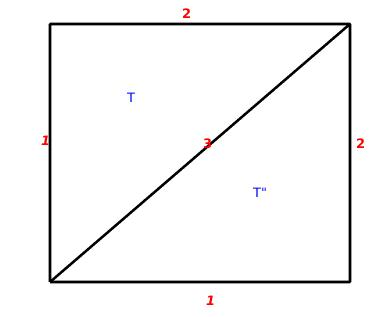
\includegraphics[width=0.35\textwidth]{figure-1.jpg}}
\caption{\small{剖分为两个单元
}} \label{logerrorandm}
\end{center}
\end{figure}

我们以上图的剖分为例来对(1.4)式进行化简:
\begin{eqnarray}
&&- \sum_{ \rm T \in \mathcal{T} }  \int _{\partial \rm T} (a \nabla u_{h}) v \cdot \vec{n_{\rm T}} dX 
\nonumber\\&& = - \int _{\partial \rm T} (a \nabla u_{h}) v \cdot \vec{n_{\rm T}} dX -  \int _{\partial \rm T^{\prime\prime}} (a \nabla u_{h}) v \cdot \vec{n_{\rm T^{\prime\prime}}} dX 
\nonumber\\&& = - \int _{e_{1}^{\rm T}} (a \nabla u)v \cdot \vec{n_{\rm T , 1}} dX -  \int _{e_{2}^{\rm T}} (a \nabla u)v \cdot \vec{n_{\rm T , 2}} dX
\nonumber\\&& = - \int _{e_{3}^{\rm T}} (a \nabla u)v \cdot \vec{n_{\rm T , 3}} dX -  \int _{e_{1}^{\rm T^{\prime\prime}}} (a \nabla u)v \cdot \vec{n_{\rm T^{\prime\prime} , 1}} dX
\nonumber\\&& =  - \int _{e_{2}^{\rm T^{\prime\prime}}} (a \nabla u)v \cdot \vec{n_{\rm T^{\prime\prime} , 2}} dX -  \int _{e_{3}^{\rm T^{\prime\prime}}} (a \nabla u)v \cdot \vec{n_{\rm T^{\prime\prime} , 3}} dX
\nonumber\\&& = -\int _{\gamma} \left\lbrace (a\nabla u_{h})| _{\rm T}  \cdot \vec{n_{\rm T , 3}}   + (a\nabla u_{h})| _{\rm T^{\prime\prime}}  \cdot \vec{n_{\rm T^{\prime\prime} , 3}}  \right\rbrace vdX
\nonumber\\&& = -\int _{\gamma} \left[ (a\nabla u_{h}) \cdot \vec{n_{\gamma}} \right]v dX,
\label{A1anotherboun}
\end{eqnarray}
其中记: $$\left[ (a\nabla u_{h}) \cdot \vec{n_{\gamma}} \right] = (a\nabla u_{h})| _{\rm T}  \cdot \vec{n_{\rm T , 3}}  +  (a\nabla u_{h})| _{\rm T^{\prime\prime}}  \cdot \vec{n_{\rm T^{\prime\prime} , 3}} ,$$
把(1.5)式推广到多单元的情况下然后代入到(1.4)式则有:
\begin{eqnarray}
&& B(e_{h},v)=\sum_{ \rm T \in \mathcal{T} }  \left\lbrace  \int _{\rm T } (f+ \nabla \cdot (a \nabla u_{h}) )v dX  - \int _{\partial \rm T} (a \nabla u_{h}) v \cdot \vec{n_{\rm T}} dX \right\rbrace
\nonumber\\&& = \sum_{ \rm T \in \mathcal{T} }   \int _{\rm T } (f+ \nabla \cdot (a \nabla u_{h}) )v dX -         \sum_{ \gamma \in \varepsilon _{I} } \int _{\gamma} \left[ (a\nabla u_{h}) \cdot \vec{n_{\gamma}} \right]v dX
\nonumber\\&& = \sum_{ \rm T \in \mathcal{T} }   \int _{\rm T } rv dX +        \sum_{ \gamma \in \varepsilon _{I} } \int _{\gamma}RvdX,
\label{A1anotherboun}
\end{eqnarray}
其中:$\varepsilon_{I}$为内部边的集合, $$ r =f+ \nabla \cdot (a \nabla u_{h}) , R = -\left[ (a\nabla u_{h}) \cdot \vec{n_{\gamma}} \right] .$$

对于给定的 $ v \in H_{0}^{1}$,令$I_{h}v$是$v$在$V_{h}$上的插值,由正交性$B(e_{h},I_{h}v)=0$则知:
\begin{eqnarray}
&& B(e_{h},v)= B(e_{h},v-I_{h}v) 
\nonumber\\&& = \sum_{ \rm T \in \mathcal{T} }   \int _{\rm T } r(v-I_{h}v) dX +        \sum_{ \gamma \in \varepsilon _{I} } \int _{\gamma}R(v-I_{h}v)dX,
\label{A1anotherboun}
\end{eqnarray}
令$v = e_{h} $则有:
\begin{eqnarray}
&& B(e_{h},e_{h})= B(e_{h},v-I_{h}e_{h}) 
\nonumber\\&& = \sum_{ \rm T \in \mathcal{T} }   \int _{\rm T } r(e_{h}-I_{h}e_{h}) dX +        \sum_{ \gamma \in \varepsilon _{I} } \int _{\gamma}R(e_{h}-I_{h}e_{h})dX
\nonumber\\&& \leq \sum_{ \rm T \in \mathcal{T} } || r|| _{L^{2}(\rm T)} \cdot || e_{h} - I_{h}e_{h} || _{L^{2}(\rm T)} + \sum_{ \gamma \in \varepsilon_{I} } || R|| _{L^{2}(\gamma)} \cdot || e_{h} - I_{h}e_{h} || _{L^{2}(\gamma)}.
\label{A1anotherboun}
\end{eqnarray}

\begin{theorem}
若剖分是拟一致的,函数$u \in W^{m+1,p}(\Omega) , 1 \leq p \leq \infty$则$u$的$m$次插值$I_{m}u$在单元$e$上有误差估计:
$$||u-I_{m}u||_{l,p,\Omega} \leq ch^{m+1-l} ||u ||_{m+1,p,\Omega},l=0,1,1\leq p \leq \infty.$$
\end{theorem}

利用定理1.1则可以得出:
\begin{equation}
||e_{h} - I_{h}e_{h}||_{L^{2}(\rm T)} \leq ch_{T} ||e_{h}||_{H^{1}(\rm T)}   ,
\end{equation}
由 $$||e_{h} - I_{h}e_{h} ||_{L^{2}(\gamma)} \leq c ||e_{h} - I_{h}e_{h} ||_{H^{1/2}(\rm T)}, $$
因:
$$||e_{h}-I_{h}e_{h}||_{H^{1/2}(\rm T)} \leq c \sqrt{h} ||e_{h}||_{H^{1}(\rm T)},$$
则:
\begin{equation}
||e_{h} - I_{h}e_{h} ||_{L^{2}(\gamma)} \leq c \sqrt{h} ||e_{h}||_{H^{1}(\rm T)}.
\end{equation}

把(1.9)(1.10)式代入到(1.8)式则有:
\begin{eqnarray}
&& B(e_{h},e_{h})
\nonumber\\&& \leq \sum_{ \rm T \in \mathcal{T} } || r|| _{L^{2}(\rm T)} \cdot || e_{h} - I_{h}e_{h} || _{L^{2}(\rm T)} + \sum_{ \gamma \in \varepsilon_{I} } || R|| _{L^{2}(\gamma)} \cdot || e_{h} - I_{h}e_{h} || _{L^{2}(\gamma)}
\nonumber\\&& \leq \sum_{\rm T \in \mathcal{T} } ||r||_{L^{2}(\rm T)} \cdot ch_{T} ||e_{h}||_{H^{1}(\rm T)}+ \sum_{\gamma \in \varepsilon_{I}} ||R||_{L^{2}(\gamma)} \cdot c \sqrt{h_{\rm T}} ||e_{h}||_{H^{1}(\rm T)}
\nonumber\\&& \leq c\left[ \left(\sum _{\rm T \in \mathcal{T}}||r||_{L^{2}(\rm T)}^{2} h_{\rm T}^{2}\right ) \cdot \left(\sum _{\rm T \in \mathcal{T}}||e_{h}||_{H^{1}(\rm T)}^{2}\right )  \right]^{1/2} 
\nonumber\\&& \hspace*{0.5cm}+ c \left[ \left (\sum _{\gamma \in \varepsilon_{I}}||R||_{L^{2}(\rm T)}^{2} h_{\rm T}\right ) \cdot \left (\sum _{\gamma \in \varepsilon_{I}}||e_{h}||_{H^{1}(\rm T)}^{2}\right )  \right]^{1/2}
\nonumber\\&& \leq c \left (\sum _{\rm T \in \mathcal{T}} ||e_{h}||_{H^{1}(\rm T)}^{2}\right )^{1/2} \left[ \left(\sum _{\rm T \in \mathcal{T}}||r||_{L^{2}(\rm T)}^{2}h_{\rm T}^{2}\right)^{1/2} +\left (\sum _{\gamma \in \varepsilon_{I}}||R||_{L^{2}(\rm T)}^{2} h_{\rm T}\right )^{1/2}  \right]
\nonumber\\&& = c \left ( ||e_{h}||_{H^{1}(\Omega)}^{2}\right )^{1/2} \left[ \left(\sum _{\rm T \in \mathcal{T}}||r||_{L^{2}(\rm T)}^{2}h_{\rm T}^{2}\right)^{1/2} +\left (\sum _{\gamma \in \varepsilon_{I}}||R||_{L^{2}(\rm T)}^{2} h_{\rm T}\right )^{1/2}  \right]
\nonumber\\&& \leq c  ||e_{h}||_{H^{1}(\Omega)}\left[ \left(\sum _{\rm T \in \mathcal{T}}||r||_{L^{2}(\rm T)}^{2}h_{\rm T}^{2}\right) +\left (\sum _{\gamma \in \varepsilon_{I}}||R||_{L^{2}(\rm T)}^{2} h_{\rm T}\right )  \right]^{1/2},
\label{A1anotherboun}
\end{eqnarray}
由 $$||e_h||_{H^{1}(\Omega)} \leq c||e_{h}||_{E},$$
则知:
\begin{eqnarray}
&& ||e_{h}||_{E}^{2} \leq c \left( \sum _{\rm T \in \mathcal{T}} ||r||_{L^{2}(\rm T)}^{2} h_{\rm T}^{2} + \sum _{\gamma \in \varepsilon _{I}} ||R||_{L^{2}(\gamma)}^{2}h_{\rm T} \right)
\nonumber\\&& =\sum _{\rm T \in \mathcal{T}}\left( h_{\rm T }^{2} ||r||_{L^{2}(\rm T)}^{2} + \dfrac{1}{2} h_{\rm T} ||R||_{L^{2}(\partial \rm T)}^{2}      \right).
\end{eqnarray}
式(1.12)中除了常数$c$都可以由数值解$u_{h}$直接解出.

则$H^{1}$型的局部误差估计子为: 
\begin{equation}
\eta _{\rm T , H^{1}}^{2} = h_{\rm T}^{2} ||r||_{L^{2}(\rm T)}^{2} + \dfrac{1}{2} h_{\rm T} ||R||_{L^{2}(\partial \rm T )}^{2}.
\end{equation}

误差估计子的可靠性:当$\eta _{\rm T , H^{1}}$小时,真实误差$e_{h}$也小.

误差估计子的有效性:真实误差$e_{h}$也从局部误差估计子从下界确定.
\subsection{显式$L^{2}$型误差估计子}
考虑模型(1.2)式的对偶问题,找$\Phi_g \in V$使得: 
\begin{equation}
B(v,\Phi _g) = (g,v)~~~~\forall v \in V.
\end{equation}

根据$||u||_{H^2} \leq C ||v||_{L^{2}}$从而得出:
\begin{equation}
||\Phi_g||_{H^2} \leq ||g||_{L^{2}}.
\end{equation}

选$g=e_h$代入到(1.14)式则有:$$||e_h||_{L^{2}(\Omega)}^{2}=B(e_h,\Phi_{e_h}),$$
带入到(1.8)式则有:
\begin{equation}
||e_h||_{L^{2}(\Omega)}^{2} \leq \sum_{ \rm T \in \mathcal{T} } || r|| _{L^{2}(\rm T)} \cdot || e_{h} - I_{h}e_{h} || _{L^{2}(\rm T)} + \sum_{ \gamma \in \varepsilon_{I} } || R|| _{L^{2}(\gamma)} \cdot || e_{h} - I_{h}e_{h} || _{L^{2}(\gamma)}
\end{equation}
由定理1.1则知:$$||e_h-I_h e_h||_{L^{2}(\rm T)} \leq ch_{\rm T}^{2}||e_h||_{H^{2}(\rm T)}$$
$$||e_h-I_h e_h||_{L^{2}(\gamma)} \leq ch^{3/2}_{\rm T} ||e_h||_{H^{2}(\gamma)}$$
代入到(1.16)式则知:
\begin{eqnarray}
&& ||e_h||_{L^{2}(\gamma)}^{2} \leq \sum_{ \rm T \in \mathcal{T} } || r|| _{L^{2}(\rm T)} \cdot ch_{\rm T}^{2}||e_h||_{H^{2}(\rm T)} + \sum_{ \gamma \in \varepsilon_{I} } || R|| _{L^{2}(\gamma)} \cdot ch^{3/2}_{\rm T} ||e_h||_{H^{2}(\gamma)}
\nonumber\\&& \leq c \left\lbrace \left( \sum_{\rm T \in \mathcal{T}} ||r||_{L^{2}(\rm T)}^{2} h_{\rm T}^{4}  \right) \cdot \left( \sum_{\rm T \in \mathcal{T}} ||e_h||_{H^{2}(\rm T)}^{2} \right)   \right\rbrace ^{\dfrac{1}{2}}
\nonumber\\&&   \hspace*{0.5cm} + c \left\lbrace \left( \sum_{\gamma \in \varepsilon_I} ||R||_{L^{2}(\gamma)}^{2} h_{\rm T}^{3}  \right) \cdot \left( \sum_{\gamma \in \varepsilon_I} ||e_h||_{H^{2}(\gamma)}^{2} \right)   \right\rbrace ^{\dfrac{1}{2}}
\nonumber\\&& \leq  c \left( \sum_{\rm T \in \mathcal{T}} ||e_h||_{H^{2}(\rm T)}^{2} \right)^{\dfrac{1}{2}} \cdot \left\lbrace \left( \sum_{\rm T \in \mathcal{T}} ||r||_{L^{2}(\rm T)}^{2} h^{4}_{\rm T}     \right)  +\left( \sum_{\gamma \in \varepsilon_{I}} ||R||_{L^{2}(\gamma)}^{2} h^{3}_{\rm T}     \right)   \right\rbrace^{\dfrac{1}{2}}
\nonumber\\&& =  c \left( ||e_h||_{H^{2}_{\Omega}}^{2}  \right)^{\dfrac{1}{2}} \cdot \left\lbrace \left( \sum_{\rm T \in \mathcal{T}} ||r||_{L^{2}(\rm T)}^{2} h^{4}_{\rm T}     \right)  +\left( \sum_{\gamma \in \varepsilon_{I}} ||R||_{L^{2}(\gamma)}^{2} h^{3}_{\rm T}     \right)   \right\rbrace^{\dfrac{1}{2}}
\nonumber\\&& \leq c  ||e_h||_{H^{2}_{\Omega}}  \cdot \left\lbrace \left( \sum_{\rm T \in \mathcal{T}} ||r||_{L^{2}(\rm T)}^{2} h^{4}_{\rm T}     \right)  +\left( \sum_{\gamma \in \varepsilon_{I}} ||R||_{L^{2}(\gamma)}^{2} h^{3}_{\rm T}     \right)   \right\rbrace^{\dfrac{1}{2}}
\nonumber\\&& \leq c \left\lbrace \left( \sum_{\rm T \in \mathcal{T}} ||r||_{L^{2}( \rm T)}^{2} h^{4}_{\rm T}     \right)  +\left( \sum_{\gamma \in \varepsilon_{I}} ||R||_{L^{2}(\gamma)}^{2} h^{3}_{\rm T}     \right) \right\rbrace 
\nonumber\\&& \leq c \sum_{\rm T \in \mathcal{T}} \left\lbrace  ||R||_{L^{2}}^{2} h_{\rm T}^{3} + ||r||_{L^{2}(\partial \rm T)}^{2} h_{\rm T}^{4}   \right\rbrace
\label{A1anotherboun}
\end{eqnarray}
则$L^{2}$型的误差估计子为:$$\eta _{\rm T,H^{1}}^{2} = ||R||_{L^{2}}^{2} h_{\rm T}^{3} + ||r||_{L^{2}(\partial \rm T)}^{2} h_{\rm T}^{4}.  $$

\section{网格生成和网格优化}
\subsection{协调的CVDT网格}
考虑求解区域$\Omega \in \mathbb{R}^{d}$是一个凸的多边形区域,$\left\lbrace X_{i} \right\rbrace _{i=1}^{n} \subset \Omega$表示特定点的集合,相对应的泰森多边形区域为$V_{i},~i=1,...,n$,~~$V_{i}$的定义为:$$V_{i} = \left\lbrace X \in \Omega| ||X-X_{i}|| < ||X-X_{j}|| ~for~ j=1,...,n~ and~ j \neq 1   \right\rbrace ,$$
显而我们有: $X_{i} \in V_{i},~V_{i} \cap V_{j} = \emptyset ~ for ~ i \neq j,~ \bigcup\limits _{i=1}^{n} \overline{V_{i}} = \overline{\Omega},$
即:$\left\lbrace V_{i}  \right\rbrace _{i}^{n}$是区域$\Omega$的曲面细分.

结合点集$\left\lbrace X_{i} \right\rbrace _{i=1}^{n}$的$\left\lbrace V_{i} \right\rbrace _{i=1}^{n}$是区域$\Omega$的泰森多边形细分.

点$\left\lbrace X_{i} \right\rbrace$称为一个生成器,子域$V_{i} \subset \Omega$称为对应于生成器的泰森多边形区域.

总所周知:对泰森多边形域对偶细分就是德劳奈三角形.

易证:泰森多边形域$V_{i}$的顶点就是德劳奈三角单元的外接圆心.

给定一个在区域$\Omega$上的密度函数$\rho (x)$,对$\forall V \subset \Omega$定义质心$X^{*}$:$$X^{*}=\dfrac{\int _{v}y \rho (y)dy}{\int _{v} \rho(y)dy}.$$

{\bf 定义1~~}CVT(Centroidal Voronoi Tessellation):当且仅当,作为泰森多边形区域$V_{i}$相对应的生成器$X_{i}$同时也是这个区域的质心,即:$$\left\lbrace (X_{i},V_{i})  \right\rbrace_{i=1}^{n} ~~if~and ~ only~ if  ~~ X_{i} = X_{i}^{*} ~~for ~~i=1,...,n,$$
相应的德劳奈三角剖分就是CVDT(Centroidal Voronoi-Delaunay triangualtion)

注意:CVT/CVDT剖分是唯一的.

能量的定义:给定$\Omega$上的点$\left\lbrace \widetilde{X_{i}}  \right\rbrace_{i=1}^{n}$ 和$\Omega$上面的一些曲面细分$\left\lbrace \widetilde{V_{i}}  \right\rbrace_{i=1}^{n}$我们给定能量的定义: $$\mathcal{K}\left(\left\lbrace \left(\widetilde{X},\widetilde{V}\right)  \right\rbrace _{i=1}^{n}\right)= \sum _{i=1}^{n} \int _{\widetilde{V_{i}}} \rho (y)||y-\widetilde{X_{i}}||^{2}dy.$$

可以证明:$\left\lbrace \left( \widetilde{X_{i}},\widetilde{V_{i}} \right) \right\rbrace_{i=1}^{n}$是CVT时,能量$\mathcal{K}$是最小的.

CVT的重要性质:能量$\mathcal{K}$以渐进的方式在泰森多边形区域$V_{i}$上均匀分布.

在一维的情况下: $$\mathcal{K}_{V_i}\approx \mathcal{K}/n~for~i=1,2...,n,$$
其中 $\mathcal{K}_{V_i} = \int _{V_i} \rho(x) ||X-X_i||^2dx$和$\mathcal{K}=\sum _{i=1}^{n} \mathcal{K}_{V_{i}}.$

这种性质在高维的情况下目前仅仅只是一个假设,但有效性已经通过大量的数值研究得到了验证.

CVT重要的几何性质:

对于一个常值密度函数,生成器$\left\lbrace X_i \right\rbrace _{i=1}^{n}$是均匀分布的;泰森多边形区域$\left\lbrace V_i \right\rbrace _{i=1}^{n}$几乎是等尺寸的.在二维的情况下,其中大部分(几乎)是全等的凸六面体.

对于一个非常值密度函数,生成器$\left\lbrace X_i \right\rbrace_{i=1}^{n}$ 是渐进局部均匀分布的,对于一些常数$c$
$$\mathcal{K}_{V_i}=c \rho (X_i) h_{V_i}^{d+2},~~\dfrac{h_{V_i}}{h_{V_j}}=\left( \dfrac{\rho (X_j)}{\rho (X_i)}  \right)^{\dfrac{1}{d+2}},$$
其中,$h_{V_i}$:$V_i$的直径;~~$d$:$\Omega$的直径.
\begin{algorithm}
 \caption{(Lloyd's method for CVT)给定一个区域$\Omega$,定义在$\Omega$上的密度函数$\rho (x)$,一个正整数$n$}

0.在$\Omega$中选定$n$个初始点$\left\lbrace X_i \right\rbrace_{i=1}^{n}$.

1.结合$\left\lbrace X_i \right\rbrace_{i=1}^{n}$产生区域$\Omega$上的泰森多边形区域$\left\lbrace V_i \right\rbrace _{i=1}^{n}$.

2.确定泰森多边形域$\left\lbrace V_i \right\rbrace_{i=1}^{n}$上的质心,这些质心产生新的点集$\left\lbrace X_i \right\rbrace_{i=1}^{n}$.

3.如果这些点满足一些收敛标准,返回$\left\lbrace \left( X_i,V_i  \right)  \right\rbrace_{i=1}^{n}$并且终止,否则转step1.
\end{algorithm}
注: $\left\lbrace \left( X_i,V_i  \right) \right\rbrace _{i=1}^{n}$的能量$\mathcal{K}$随着每次迭代减少.

{\bf 记号:}
\begin{itemize}
\item $P_S = \left\lbrace  Z_i \right\rbrace_{i=1}^{k}$:求解区域的角顶点
\item $P_I=\left\lbrace X_i|\overline{V_i} \cap \partial \Omega = \emptyset  \right\rbrace$:内部点的集合
\item $P_B=\left\lbrace X_i | \overline{V_i} \cap \partial \Omega \neq  \emptyset  \right\rbrace $:边界点的集合
\item $Proj(X):$表示将点$X$投影到离$X$最近边界上的点.
\end{itemize}
{\bf 定义2~~}一个$\Omega$上的泰森多边形区域细分$\left\lbrace \left( X_i,V_i \right) \right\rbrace_{i=1}^{n}$被称为一致重心的泰森多边形细分(CfCVT)当且仅当下面的性质被满足:
\begin{itemize}
\item $P_S \subset \left\lbrace X_i \right\rbrace_{i=1}^{n},$
\item $X_i = X_{i}^{*}~for ~ X_i \in P_I,$
\item $X_i = Proj(X_{i}^{*}) ~for ~ X_i \in P_B - P_S,$
\end{itemize}
相应的对偶剖分为(CfCVDT).

\begin{algorithm}
 \caption{~~constructing a CfCVT/CfCVDT}

0.在$\Omega$中选定$n$个初始点$\left\lbrace X_i \right\rbrace_{i=1}^{n}$.

1.结合$\left\lbrace X_i \right\rbrace_{i=1}^{n}$产生区域$\Omega$上的泰森多边形区域$\left\lbrace V_i \right\rbrace _{i=1}^{n}$.

2.确定泰森多边形域$\left\lbrace V_i \right\rbrace_{i=1}^{n}$上的质心,这些质心产生新的点集$\left\lbrace X_i \right\rbrace_{i=1}^{n}$.

3.除非边界泰森多边形区域包含$P_B$中的一点,否则就把边界泰森多边形区域的质心投影到边界上,这个一点就是新的生成器.

4.如果这些点满足一些收敛标准,返回$\left\lbrace \left( X_i,V_i  \right)  \right\rbrace_{i=1}^{n}$并且终止,否则转step1.
\end{algorithm}
\subsection{近似CfCVD构造}
\begin{itemize}
\item CDTs:受限的德劳奈三角剖分
\item CDT过程产生初始的三角剖分 $\mathcal{T}_{0} = \left\lbrace \rm T _{i} \right\rbrace _{i=1}^{m}$
\item $P_S = \left\lbrace Z \right\rbrace _{i=1}^{k}$:区域角顶点
\item $P = \left\lbrace X_i \right\rbrace _{i=1}^{n}$:$\mathcal{T}$的顶点的集合
\item $P_B$:边界点的集合
\item $P_I$:内部点的集合
\item $\overline{X}_i$:在泰森多边形区域$U_i$上符合密度函数$\rho(x)$的质心
\end{itemize}
CDT过程保证:$P_S \subset P_B.$

{\bf 定义3}~~对于每一个三角单元$\rm T_{i} = \left( X_{i1},X_{i2},X_{i3} \right) \in \mathcal{T}_{0}$定义:
\begin{equation}
    X_{\rm T_i}=
   \begin{cases}
   circumcenter~of~\rm T_i &\mbox{if $\rm T_i$ is an acute triangle}\\
   the~middle~point~of~the~longest~edge~of~\rm T_i&\mbox{otherwise}
   \end{cases}
\end{equation}
很明显有$X_{\rm T_i} \in \overline{\rm T}_{i}$

{\bf 内部点.} ~~	当$X_i$是内部点的时候定义$U_i$(泰森多边形区域):
$$U_i = the~ polygon~formed~by~\left\lbrace X_{\rm T_{i_k}} \right\rbrace _{k=1}^{m};$$
\begin{itemize}
\item $\left\lbrace \alpha_{i_k} \right\rbrace_{k=1}^{m_i}$:围绕点$X_i$相应$\left\lbrace \rm T_{i_k} \right\rbrace_{k=1}^{m_i}$的角度;
\item
\begin{equation}
   \alpha=
   \begin{cases}
   max \left\lbrace \alpha_{i_k}| \overline{\rm T}_{i_k} \cap \partial \Omega \neq 0  \right\rbrace  &\mbox{if $\overline{\rm T}_{i_k} \cap \partial \Omega \neq 0$ for some $i_k$}\\
   0 &\mbox{otherwise;}
   \end{cases}
\end{equation}
\item 令$e_i$表示与角度$\alpha_{i_k}$相对应的边界边缘,使得:$\alpha _{i_k}=\alpha$;
\end{itemize}
选择参数$\theta_{max}(\pi) > \theta_{max} > \pi / 2$,定义:
\begin{equation}
   y_i=
   \begin{cases}
  \overline{X_i}  &\mbox{if $\alpha < \theta_{max}$}\\
   Proj_{e_i}X_i &\mbox{otherwise;}
   \end{cases}
\end{equation}
其中$Proj_{e_i}X_i$表示将$X_i$投影到边界边$e_i$上,显而可知当$\alpha < \theta_{max}$时$y_i$都是内部点.

{\bf 边界点.}~~当$X_i$是边界点的时候,
\begin{itemize}
\item 令$e_1$和$e_2$表示具有$X_i$作为公共端点的两个边界边缘;
\item 泰森多边形区域$U_i$定义为:$$U_i = the~polygon~formed~by~Z_1,\left\lbrace X_{\rm T_{i_k}} \right\rbrace_{k=1}^{m_i},Z_2;$$
\item 如果$X_i \in P_B - P_S$,定义$\beta_1$和$\beta_2$分别是对应边$e_1$和$e_2$的角度;
\item $\beta = max(\beta_1,\beta_2);$
\item 当参数$\theta_{min}(\pi/3 > \theta_{min} > 0)$,定义:
\begin{equation}
   y_i=
   \begin{cases}
  X_i  &\mbox{if $ X_i \in P_S$}\\
   Proj_{\overline{Z_1Z_2}}X_i &\mbox{if $X_i \in P_B - P_S$~and~$\beta > \theta_{min}$}\\
   \overline{X_i} &\mbox{if $X_i \in P_B - P_S$~and~$\beta \leq \theta_{min},$}
   \end{cases}
\end{equation}
其中$Proj_{\overline{Z_1Z_2}}X_i$表示将$X_i$投影到$\overline{Z_1Z_2}$上;
\end{itemize}

\begin{algorithm}
 \caption{~~modified Lloyd method for approximate CfCVDT}
给定一个求解域$\Omega$,在$\Omega$上定义密度函数$\rho(x)$,以及使用CDT在求解域$\Omega$上生成具有顶点$\left\lbrace X_i \right\rbrace_{i=1}^{n}$的初始三角剖分$\mathcal{T}_0$.

1.根据(2.16)和(2.17)从$\left\lbrace X_i \right\rbrace_{i=1}^{n}$确定$\left\lbrace y_i \right\rbrace_{i=1}^{n}$.

2.集合$\left\lbrace X_i \right\rbrace_{i=1}^{n} = \left\lbrace y_i \right\rbrace_{i=1}^{n}$,从新的$\left\lbrace X_i \right\rbrace_{i=1}^{n}$重建边界段$\varepsilon _B$.

3.把$\left\lbrace X_i  \right\rbrace_{i=1}^{n}$作为顶点和$\varepsilon_B$作为边界边,使用CDT对区域$\Omega$重新进行三角剖分.

4.如果三角剖分$\mathcal{T}$满足一些收敛标准,返回$\mathcal{T}$并且终止,否则转step1.
\end{algorithm}

注:
\begin{itemize}
\item 为了防止一些顶点频繁的在边界和内部之间跳动,需要更复杂的控制,为了简单起见省略了上述算法的一些细节.
\item 取$\theta_{max}=5\pi/9$和$\theta_{min}=\pi/6.$
\end{itemize}





\end{CJK}
\end{document}
